% ****************************************************************************************************
\chapter[Business Models of Platform as a Service Providers -- Current State]{Business Models of Platform as a Service\protect\linebreak Providers -- Current State}\label{ch:sota}
% ****************************************************************************************************

In order to assess the current state of \ac{PaaS} providers' business models and identify key elements within these business models, the current business models of 23 \ac{PaaS} providers were analyzed. The initial selection of the analyzed \ac{PaaS} providers in this thesis was based on technical reports respectively market reports provided by three different market research companies:
\begin{itemize}[parsep=0pt, topsep=0pt, itemsep=0pt]
	\item Forrester Research, Inc. -- \citet{Rymer2011,Ried2011a}
	\item \ac{IDC} -- \citet{Bradshaw2012,Hendrick2012, Hendrick2012a}
	\item Gartner, Inc. -- \citet{Smith2012}
\end{itemize}
The initially identified and selected \ac{PaaS} providers were further selected to receive a manageable set of representative \ac{PaaS} providers. Four disjunct selection criteria were used in the second evaluation round to identify the final set of 23 \ac{PaaS} providers, viz (1) market share, (2) growth rate, (3) availability of the platform to customers as of February 2013, and (4) background of the \ac{PaaS} provider, for instance, former purely \ac{IaaS} or \ac{SaaS} providers extend their cloud portfolio with \ac{PaaS} functionalities. According to \citet{Hendrick2012}, the world largest \ac{PaaS} provider is GXS Worldwide, Inc. (cf. Appendix \ref{ch:app01:gxs}) with a market share of 14.2\% in 2011 and with a growth rate of 428.6\% in 2011 CloudBees  is the fastest-growing \ac{PaaS} provider (cf. Subsection \ref{ch:sota:cb}).

In the first part of this chapter four case studies -- CloudBees, GigaSpaces Cloudify, Facebook Developers, and SAP HANA Cloud -- are described representatively in detail. To receive a coherent representation, all investigated business models within this thesis follow the prior introduced business model conceptualization approach (cf. Subsection \ref{ch:tf:bmc}). The remaining 19 case studies are presented for reasons of comprehensibility within Appendix \ref{ch:app01}. All 23 presented cases studies are based on data available as of February 2013. Based upon the performed analysis of current \ac{PaaS} providers' business models, a classification scheme for \ac{PaaS} providers was developed and is introduced in Section \ref{ch:sota:cm}. At the end of this chapter an overview of all investigated \ac{PaaS} providers by the use of the developed classification scheme is provided as well as shortly discussed.

%In the first part of this chapter four case studies -- CloudBees, GigaSpaces Cloudify, Facebook Developers, and SAP Hana Cloud -- are described representatively in detail. The remaining 19 case studies are presented for reasons of comprehensibility within Appendix \ref{ch:app01}. All 23 presented cases studies are based on data available as of February 2013. To receive a coherent representation, all presented business models within this thesis follow the prior introduced business model conceptualization approach (cf. Subsection \ref{ch:sota:bmc}). Based upon the performed analyzes of current \ac{PaaS} providers' business models, a classification scheme for \ac{PaaS} providers was developed and is introduced in Section \ref{ch:sota:cm}. At the end of this chapter an overview of all investigated \ac{PaaS} providers by the use of the developed classification scheme is provided as well as shortly discussed.

\section{Representative Case Studies}

The main focus at all conducted case studies was rather how these business models appear on the market and are experienced by their customers than how these business models are implemented by a specific company or to describe the internal view of these business models. For this reason, the market view elements -- the \ac{CVP} and, in parts, the profit formula -- are mainly considered, even though the non-market view elements -- key resources and key processes -- are mentioned as far as possible. Moreover, the focus on market view elements allowed to solely utilize secondary data for the conducted analysis of \ac{PaaS} providers' business models -- for instance reliable, public data or documentations, both providing comprehensive information about the business model under investigation. Information concerning the internal business model elements -- key resources, key processes, and, in parts, the profit formula -- is difficult to obtain, due to the fact, that this information is in most cases kept confidential, for instance, the cost structure as well as process or workflow descriptions. Thus, the following presented business models mainly focus on the market view elements.

\subsection{The Case of CloudBees}\label{ch:sota:cb}

CloudBees was founded in the beginning of 2012 and introduced its identically named \ac{PaaS} offer. Many members of CloudBees' management team, including the founder, worked prior for companies like Oracle, Sun, IBM, and VMware or were involved in development projects around JBoss and Jenkins CI. Already the background of CloudBees' management reveals the main objective -- a \ac{PaaS} solution truly dedicated around the Java programming language ecosystem, supporting the whole application lifecycle \citep{CloudBees2013}.

The CloudBees platform is composed of two distinct but related concepts. First, all development, integration, and testing tasks are performed within the DEV@cloud. Core of this part of the platform is the Jenkins Continuous Integration server. Once an application is ready to go live, the application is migrated to the RUN@cloud. Basically, the RUN@cloud represents a traditional application server, including the functionalities load balancing, scalability, and high availability, based on various cloud infrastructures.

Mainly two different customer groups are attracted by CloudBees platform solution -- business end-consumer and \acp{ISV}. The first-mentioned group utilizes the platform to manage the entire application lifecycle -- including development, quality assurance and testing, deployment and release management, as well as monitoring and administration. Due to the fact, that all applications upon the CloudBees platform are based on standard Java and not on specific CloudBees \acp{API}, potential customers are not faced with a so-called lock-in effect. Moreover, platform customers can select between multi-tenant and dedicated RUN@cloud's. In case of dedicated instances, they can choose the appropriate cloud infrastructure -- private, public, and hybrid provisioning scenarios are supported. Via the CloudBees Partner Ecosystem, business end-consumer can purchase third-party applications and services and extend the CloudBees platform functionalities. 

Platform extensions are provided by the second customer group, the \acp{ISV}. CloudBees uniquely defined mission -- support the whole application lifecycle for standard Java and \ac{JVM} based applications within the cloud -- enables \acp{ISV} to expand the already existing platform capabilities by deployment and testing tools, comprehensive monitoring features, as well as different databases. All third-party applications, tools, and services are listed within the CloudBees Partner Ecosystem. Especially for small \acp{ISV}, but certainly also for all other \acp{ISV}, it is beneficial, that the payment handling, inclusive billing, for third-party extensions is performed by CloudBees.

The overall revenue of CloudBees is composed of two revenue streams -- through CloudBees' partners and CloudBees' platform customers. Consulting partners, i.e. \acp{SI}, need to pay an annual partner fee -- silver partners 2.000 \ac{USD} and gold partners 5.000 \ac{USD} -- to become a certified CloudBees Service Partner. For all third-party applications, tools, and services provided by \acp{ISV}, denoted by CloudBees as Technology Partners, CloudBees gets a default revenue share of 30\%. Nevertheless, CloudBees offers the possibility to negotiate the revenue share rate individually.

Business end-consumer pay for the CloudBees platform a combination of subscription and transaction based fees. The DEV@cloud is available as four different packages -- Free 0 \ac{USD}, Base 15 \ac{USD}, Pro 50 \ac{USD}, and Enterprise 100 \ac{USD}, all prices per month -- including different features and quotas. A different number of build minutes is included within all packages and additional build minutes can be purchased for 0.106 \ac{USD} respectively 0.425 \ac{USD} per hour. A multi-tenant RUN@cloud is either free (no additional features or services can be purchased) or charged per hour, based on the select application server and SSL connections. As mentioned above, the dedicated RUN@cloud can basically be hosted at any cloud infrastructure, with the result that a vast number of pricing models is possible. For instance, the CloudBees RUN@cloud platform hosted at \ac{AWS} infrastructure is priced between 153 - 644 \ac{USD} per instance monthly. Furthermore, CloudBees is offering also a MySQL database which is priced based on the selected RUN@cloud \citep{CloudBees2013}. Please find an illustration of the above discussed business model within Table \ref{bm:cloudbees}:

% ****************************************************************************************************
% Business Model CloudBees NEW
% ****************************************************************************************************
\begin{longtable}{L{\column}L{\column}L{\column}L{\column}}
	
	\caption[Business Model CloudBees]{Business Model CloudBees \citep{CloudBees2013}}
	\label{bm:cloudbees}\\
	
	\toprule
	\multicolumn{4}{l}{\footnotesize \textit{\nameref{bm:cloudbees}}}\\ 
	\midrule
	\endfirsthead
	\toprule  
	\multicolumn{4}{l}{\footnotesize \textit{continued from previous page (\nameref{bm:cloudbees})}}\\ 
	\midrule
	\endhead
	\multicolumn{4}{r}{\footnotesize \textit{continued on next page}}\\
	\bottomrule
	\endfoot
	\bottomrule
	\endlastfoot
	
	\multicolumn{4}{c}{\small \textbf{Customer Value Proposition (CVP)}}\\ \midrule
	
	\footnotesize Target customer &
	\footnotesize Job to be done &
	\multicolumn{2}{L{\columnT}}{\footnotesize Offering} \\ \midrule
	
	% START CUSTOMERS
	\footnotesize
	Business End-Consumer &
	\footnotesize
	Manage the entire Java application lifecycle within the cloud in a cost efficiency manner & 
	\multicolumn{2}{L{\columnT}}{
	\vspace{-5mm}
	\footnotesize
	\begin{itemize}[leftmargin=*, parsep=0pt, topsep=0pt, itemsep=0pt]
				\item Manage the entire Java and \ac{JVM} application lifecycle
				\item CloudBees Eclipse plugin and \ac{SDK}
				\item Different deployment scenarios: public, private, and hybrid
				\item 'No vendor lock-in' (standard Java)
				\item CloudBees partner ecosystem provides platform extensions -- databases, monitoring as well as deployment tools\vspace{-\baselineskip} 
		\end{itemize}
	} \\ \midrule
	\footnotesize	
	\ac{ISV} &
	\footnotesize
	Develop, manage, and market application lifecycle related applications and services globally &
	\multicolumn{2}{L{\columnT}}{
		\vspace{-5mm} 
		\footnotesize
		\begin{itemize}[leftmargin=*, parsep=0pt, topsep=0pt, itemsep=0pt]
				\item CloudBees platform as a service truly dedicated to Java and \ac{JVM} applications (clear mission)
				\item Service resp. application listing within the Ecosystem Technology Partner directory
				\item Support mechanism between CloudBees and service provider, to resolve customer problems within a narrow time frame
				\item Joint marketing activities
				\item Payment handling (incl. billing) by CloudBees\vspace{-\baselineskip} 
		\end{itemize}
	} \\ \midrule

% END CUSTOMERS

% KEY RESOURCES
\multicolumn{2}{L{\columnT}}{\small \textbf{Key Resources}
\footnotesize
\begin{itemize}[leftmargin=*, parsep=0pt, topsep=0pt, itemsep=0pt]
				\item CloudBees' platform, including
					\begin{itemize}[leftmargin=*, topsep=0pt, itemsep=0pt]
						\item Build: create, integrate, and test
						\item Run: choose, deploy, and store
						\item Manage: scale, monitor, and enhance
					\end{itemize}
				\item CloudBees Eclipse plugin and \ac{SDK}
				\item Consulting partners, for instance Black Diamond Software
				\item Partnership with \ac{IaaS} providers, for instance \ac{AWS}\vspace{-\baselineskip} 
	\end{itemize}
} &
% KEY PPROCESSES
\multicolumn{2}{L{\columnT}}{\small \textbf{Key Processes}
\footnotesize
\begin{itemize}[leftmargin=*, parsep=0pt, topsep=0pt, itemsep=0pt]
				\item Maintain full lifecycle support for Java and \ac{JVM} applications as well as keep the platform up to date (in respect of new Java versions and features)
				\item Facilitate different deployment scenarios -- public, private, and hybrid -- based on multiple \ac{IaaS} providers
				\item Maintain partnerships with existing \ac{IaaS} providers as well as begin negotiations with potential providers
				\item Partner program for consulting partners, including business and marketing support, access to products plans, trainings, reselling options, and listing in the CloudBees Service Partner Directory
				\item Offer support via Stack Overflow, \ac{FAQ}, and documentation/ guides deployment tools\vspace{-\baselineskip} 
\end{itemize}
} \\ \midrule

% PROFIT FORMULA
\multicolumn{4}{L{\columnF}}{\small \textbf{Profit Formula}
	\footnotesize
	\begin{itemize}[leftmargin=*, parsep=0pt, topsep=0pt, itemsep=0pt]
				\item Subscription and transaction based revenue for platform usage:
					\begin{itemize}[leftmargin=*, topsep=0pt, itemsep=0pt]
						\item DEV@cloud: \ac{USD} 0 - 100 / Monthly + build minutes
						\item RUN@cloud Multi-Tenant: Free (limited) or transaction based (depends among other things on the used software stack per application per hour) 
						\item RUN@cloud Dedicated: Different IaaS providers, e.g. \ac{AWS} US m1.small \ac{USD} 153 \/ Monthly
						\item Database: Offered by CloudBees (MySQL) \ac{USD} 0 - 25 / Monthly or by different partners
					\end{itemize}
				\item Partner program fee: \ac{USD} 2000 - 5000 / Yearly
				\item Revenue sharing (30\%; or individual negotiated) for applications and services offered by third parties\vspace{-\baselineskip} 
	\end{itemize}
} \\

\end{longtable}





\subsection{The Case of GigaSpaces Cloudify}\label{ch:sota:gsc}

Within the evolving \ac{PaaS} ecosystem just a few open source platform solutions are available -- Cloudify is one of them. Since the beginning of 2012, the Cloudify Open \ac{PaaS} Stack is available on the market. Cloudify itself and the Cloudify Community are promoted by the company GigaSpaces \citep{GigaSpaces2013a}.

The basic concept of Cloudify is the so-called external blueprint, also named as recipe. Within a blueprint the deployment and post-deployment activities of an application are described. This concept enables developers to migrate existing applications to cloud infrastructure without the need to adopt or change the source code. Moreover, based on the blueprint concept, applications can be deployed at or migrated between private, public, or even hybrid cloud infrastructures \citep{GigaSpaces2013a}.

Two distinct customer groups can use the Cloudify platform offer: (1) business end-consumers who want to move existing non-cloud applications to the cloud or develop and operate cloud applications and (2) \acp{ISV} who want to offer migration services (migrate on-premise applications onto cloud infrastructure). The value proposition for these two stakeholder groups include the promise to move any application without code or application architecture changes to the cloud, develop the external blueprint for an application once and be able to deploy the application at different cloud infrastructures, as well as full control over the Cloudify Open \ac{PaaS} Stack. Furthermore, an interactive shell and web-based user-interface for monitoring purposes are provided \citep{GigaSpaces2013a}.

As usual for many open source projects, a flourishing community -- here the Cloudify Community -- is actively participating around the open source product. Within the Cloudify Community product related knowledge is shared via support forums, documentations, events, blogs, and videos. Moreover, the Cloudify platform source code and sample Cloudify blueprints respectively recipes are public available via GitHub \citep{GigaSpaces2013b,GitHub2013,GitHub2013a}.

GigaSpaces' Cloudify platform is offered as an open source platform and thereby free of charge for the platform software itself. However, it should be noted that Cloudify platform users still need the corresponding cloud infrastructure, for instance offered for a fee by \ac{AWS}, Rackspace, and HPCloud. Various charged services with regard to Cloudify are provided by GigaSpaces, including technical support, trainings, and consultancy services \citep{GigaSpaces2013a}. Please find an illustration of the above discussed business model within Table \ref{bm:cloudify}:

% ****************************************************************************************************
% Business Model GigaSpaces Cloudify NEW
% ****************************************************************************************************
\begin{longtable}{L{\column}L{\column}L{\column}L{\column}}
	
	\toprule
	\multicolumn{4}{l}{\textit{\nameref{bm:cloudify}}}\\ 
	\midrule
	\endfirsthead
	\toprule
	\multicolumn{4}{l}{\textit{continued from previous page (\nameref{bm:cloudify})}}\\ 
	\midrule
	\endhead
	\multicolumn{4}{r}{\textit{continued on next page}}\\
	\bottomrule
	\endfoot
	\bottomrule
	\caption[Business Model GigaSpaces Cloudify]{Business Model GigaSpaces Cloudify \citep{GigaSpaces2013a,GigaSpaces2013b}}
	\label{bm:cloudify}
	\endlastfoot
	
	\multicolumn{4}{c}{ \textbf{Customer Value Proposition (CVP)}}\\ \midrule

	Target customer &
	Job to be done &
	\multicolumn{2}{L{\columnT}}{Offering} \\ \midrule
	
	% START CUSTOMERS
	
	\small
	Business End-Consumer &
	\small
	Operate applications in the cloud  & 
	
	\multicolumn{2}{L{\columnT}}{
	\vspace{-5mm} 
		\small
		\begin{itemize}[leftmargin=*, parsep=0pt, topsep=0pt, itemsep=0pt]
				\item Move any application (without code changes) to the cloud
				\item 'No vendor lock-in' (no specific programming language)
				\item Deployment and post-deployment steps (installing, starting, orchestrating, and monitoring) are described within a blueprint (also known as recipe)\vspace{-\baselineskip} 
		\end{itemize}
	}\\ \midrule
	
	\small
	\ac{ISV} &
	\small
	Offer migration services (on-premise onto cloud infrastructure) to customers & 
	\multicolumn{2}{L{\columnT}}{
	\vspace{-5mm} 
		\small
		\begin{itemize}[leftmargin=*, parsep=0pt, topsep=0pt, itemsep=0pt]
				\item Different deployment scenarios: public, private, and hybrid; fast migration process through blueprint concept
				\item Local testing 
				\item Full control over the platform stack
				\item Automatic scaling based on custom metrics (scale-in and scale-out)
				\item Cloudify shell \vspace{-\baselineskip} 
		\end{itemize}
	}	\\ \midrule

% END CUSTOMERS

% KEY RESOURCES
\multicolumn{2}{L{\columnT}}{ \textbf{Key Resources}
	\small
	\begin{itemize}[leftmargin=*, parsep=0pt, topsep=0pt, itemsep=0pt]
				\item Open source Cloudify platform stack
				\item Cloudify Community
				\item Blueprint resp. recipe concept
				\item Cloud Driver \ac{API}
				\item Web-based user-interface (monitoring)
				\item Cloudify shell\vspace{-\baselineskip} 
	\end{itemize}
} &
% KEY PPROCESSES
\multicolumn{2}{L{\columnT}}{ \textbf{Key Processes}
	\small
	\begin{itemize}[leftmargin=*, parsep=0pt, topsep=0pt, itemsep=0pt]
				\item Maintain, improve, and extend the blueprint/ recipe concept, the Cloud Driver \ac{API}, as well as the web-based user interface
				\item Provide instructions how to build or ready to use blueprints/ recipes, for instance how to deploy a multi-tier application on \ac{AWS} infrastructure
				\item Promote the Cloudify Community\vspace{-\baselineskip} 
	\end{itemize}
} \\ \midrule

% PROFIT FORMULA
\multicolumn{4}{L{\columnF}}{ \textbf{Profit Formula}
	\small
	\begin{itemize}[leftmargin=*, parsep=0pt, topsep=0pt, itemsep=0pt]
		\item \ac{OSS}
		\item Various charged services provided by GigaSpaces:
		\begin{itemize}[leftmargin=*, parsep=0pt, topsep=0pt, itemsep=0pt]
			\item Technical support
			\item Account and product management
			\item Education services
			\item Consultancy services for Cloudify: on-boarding support, assessments and reviews, as well as implementation projects\vspace{-\baselineskip} 
		\end{itemize}
	\end{itemize}
} \\

\end{longtable}





\subsection{The Case of Facebook Developers}\label{ch:sota:fd}

Facebook -- the social network with more than a billion monthly active users, 655 million daily active users, and 751 million monthly active users using mobile devices to access Facebook's social network; all figures as of March 2013 -- introduced its \ac{PaaS} offer, called Facebook Developers, in May 2007 \citep{Facebook2013}. By the end of March 2012, more than nine million applications and websites are built upon or utilizing features of the Facebook Developers platform and are integrated with Facebook \citep{Facebook2013}. Facebook Developers gains its attractiveness especially through Facebook's huge user base and thereby millions of potential users of applications and websites.

The Facebook Developers platform can be used to integrate Facebook features and services into (mobile) applications as well as websites. In the other direction the platform can be used to integrate (mobile) applications into Facebook. Furthermore, advertising providers provide advertisement services which can be used by developers to monetize their efforts. The Facebook Developers platform provides a comprehensive set of tools and features to support different kinds of development and administration tasks \citep{Facebook2013a}: Facebook \acp{SDK} for iOS, Android, JavaScript, and PHP; third-party \acp{API} for .NET (C\#), Falsh (ActionScript), Python, Java (Spring), Java (BlackBerry), Ruby, and Node.js; Facebook \acp{API} like Login, Graph \ac{API}, and Facebook Query Language (FQL) ; and tools like the Graph \ac{API} Explorer as well as a JavaScript Test Console. Applications are distributed over the Facebook App Center (marketplace) with linkage functionality for native mobile applications -- for iOS applications linkage to the App Store and for Android applications linkage to the Google Play Store -- as well as on-demand provisioning for non-native mobile or browser-based applications.

Facebook is generating monetary revenue mainly with the following three revenue streams. First, new or already existing applications can be promoted through a fee-based promoting self-service. Facebook offers the possibility to define the target audience -- for instance region, age, and gender --, the promoting goal -- for instance get installs --, and the promoting budget. Second, application users can purchase digital and virtual goods in social applications based on the currency Facebook Credits, since end of 2012 also the option local currency pricing is possible \citep{Facebook2013a}. In order to use in-app payment, users need to buy Facebook Credits or, in case of local currency pricing, pay directly with their credit card, PayPal, or another payment method. The application or service provider on the other side can change the Facebook Credits obtained through their applications and services into real money. Facebook takes a 30\% charge for this service. And third, most likely the most important revenue stream is generated through personalized advertisements, for instance within applications and websites.

Furthermore, Facebook generates also non-monetary revenue in respect of even more detailed and valuable user data capturing. It is possible to login to various websites and services (build with the help of features of the Facebook Developer platform) with a valid Facebook account -- a kind of single sign-on (SSO) system which can be considered as a lock-in effect and allows Facebook to collect valuable user data from various external sources. Please find an illustration of the above discussed business model within Table \ref{bm:facebook}:

\newpage
% ****************************************************************************************************
% Business Model Facebook Developers
% ****************************************************************************************************
\begin{longtable}{L{\column}L{\column}L{\column}L{\column}}
	
	\toprule
	\multicolumn{4}{l}{\textit{\nameref{bm:facebook}}}\\ 
	\midrule
	\endfirsthead
	\toprule  
	\multicolumn{4}{l}{\textit{continued from previous page (\nameref{bm:facebook})}}\\ 
	\midrule
	\endhead
	\multicolumn{4}{r}{\textit{continued on next page}}\\
	\bottomrule
	\endfoot
	\bottomrule
	\caption[Business Model Facebook Developers]{Business Model Facebook Developers \citep{Facebook2013a,Facebook2013}}
	\label{bm:facebook}
	\endlastfoot
	
	\multicolumn{4}{c}{ \textbf{Customer Value Proposition (CVP)}}\\ \midrule
	
	Target customer &
	Job to be done &
	\multicolumn{2}{L{\columnT}}{Offering} \\ \midrule
	
	% START CUSTOMERS
	\small
	\ac{ISV} &
	\small
	Develop and market browser as well as mobile applications resp. games & 
	\multicolumn{2}{L{\columnT}}{
	\vspace{-5mm}
	\small
	\begin{itemize}[leftmargin=*, parsep=0pt, topsep=0pt, itemsep=0pt]
				\item Facebook and third-party \acp{SDK}
				\item Facebook \acp{API}
				\item Income through advertisements and Facebook Credits
				\item Tools like the JavaScript Test Console
				\item Service for free
				\item Existing user base\vspace{-\baselineskip} 
		\end{itemize}
	} \\ \midrule
	\small	
	Business End-Consumer &
	\small
	Integrate social network services into (existing) applications and websites &
	\multicolumn{2}{L{\columnT}}{
		\vspace{-5mm} 
		\small
		\begin{itemize}[leftmargin=*, parsep=0pt, topsep=0pt, itemsep=0pt]
				\item Facebook and third-party \acp{SDK}
				\item Facebook \acp{API}
				\item Social Plugins
				\item Tools like the JavaScript Test Console
				\item Service for free
				\item Existing user base\vspace{-\baselineskip} 
		\end{itemize}
	} \\ \midrule
	\small	
	Advertising Broker &
	\small
	Act as an intermediary between advertisers and developers resp. application providers &
	\multicolumn{2}{L{\columnT}}{
		\vspace{-5mm} 
		\small
		\begin{itemize}[leftmargin=*, parsep=0pt, topsep=0pt, itemsep=0pt]
				\item Flourishing global ecosystem with broad user base
				\item Certification process for advertising providers
				\item Public list with all approved advertising providers\vspace{-\baselineskip} 
		\end{itemize}
	} \\ \midrule
	\small	
	Private End-Consumer &
	\small
	Participation in a social network including diverse games resp. applications &
	\multicolumn{2}{L{\columnT}}{
		\vspace{-5mm} 
		\small
		\begin{itemize}[leftmargin=*, parsep=0pt, topsep=0pt, itemsep=0pt]
				\item Facebook.com
				\item Facebook App Center
				\item Social plugins\vspace{-\baselineskip} 
		\end{itemize}
	} \\ \midrule

% END CUSTOMERS

% KEY RESOURCES
\multicolumn{2}{L{\columnT}}{ \textbf{Key Resources}
\small
\begin{itemize}[leftmargin=*, parsep=0pt, topsep=0pt, itemsep=0pt]
				\item Infrastructure
				\item Facebook.com
				\item Existing user base
				\item Facebook \acp{SDK} for iOS, Android, JavaScript, and PHP (provided by Facebook itself)
				\item Third-party \acp{SDK} for .NET (C\#), Flash (ActionScript), Python, Java (Spring), Java (BlackBerry), Ruby, and Node.js
				\item Facebook \acp{API}: Login, Graph \ac{API}, Facebook Query Language (FQL), and Ads \ac{API}
				\item Facebook App Center (marketplace) with linkage (for native applications) as well as provisioning (browser-based applications)
				\item Social Plugins: Link Button, Follow Button, Login Button and more
				\item Tools: Graph \ac{API} Explorer, JavaScript Test Console, and more\vspace{-\baselineskip} 
	\end{itemize}
} &
% KEY PPROCESSES
\multicolumn{2}{L{\columnT}}{ \textbf{Key Processes}
\small
\begin{itemize}[leftmargin=*, parsep=0pt, topsep=0pt, itemsep=0pt]
				\item Infrastructure management
				\item Linkage management between Facebook App Center and Google Play Store as well as Apple App Store
				\item Payment services for Facebook Credits: purchase (mainly by application users) and exchange (mainly by application providers)
				\item Partner program, i.e. Preferred Marketing Developer Program
				\item Maintain and publish documentations, sample applications, and best practices
				\item Offer support via Stack Overflow, Facebook Communities, and \ac{FAQ}
\vspace{-\baselineskip} 
\end{itemize}
} \\ \midrule

% PROFIT FORMULA
\multicolumn{4}{L{\columnF}}{ \textbf{Profit Formula}
	\small
	\begin{itemize}[leftmargin=*, parsep=0pt, topsep=0pt, itemsep=0pt]
				\item Monetary:
					\begin{itemize}[leftmargin=*, topsep=0pt, itemsep=0pt]
						\item Promoting service for new applications
						\item Facebook credit (also local currency pricing):
Possible use case: An application user buys equipment paid by Facebook Credits within a game. The application provider changes these credits into real money -- Facebook takes a 30\% charge.
						\item Personalized advertisements
					\end{itemize}
				\item Non-Monetary:
				\begin{itemize}[leftmargin=*, topsep=0pt, itemsep=0pt]
						\item Detailed and valuable user data
					\end{itemize}\vspace{-\baselineskip} 
	\end{itemize}
} \\

\end{longtable}





\subsection{The Case of SAP HANA Cloud}\label{ch:sota:sap}

SAP, a German enterprise software vendor with more than 200.000 customers worldwide, launched a new \ac{PaaS} solution -- named SAP HANA Cloud -- at the end of 2012 \citep{SAP2013b,SAP2013a}. SAP HANA Cloud aims to support the development, deployment, and management of standalone as well as integrated cloud applications. The platform itself and the applications build upon the platform are both hosted by SAP with a guaranteed system availability of 99.9\% \citep{SAP2013b}.

SAP's new \ac{PaaS} solution is targeting four diverse stakeholder groups. Application customers who want to use pure \ac{SaaS} applications as well as complement existing SAP and non-SAP on-premise systems with cloud applications, build the first customer group. Presumably the most important part of SAP's offer for this stakeholder group, is the SAP Store with certified third-party applications (ensured quality assurance) and the guaranteed system availability of 99.9\%.

Development partners -- the second stakeholder group -- utilize the platform to develop, deploy, manage, and market business \ac{SaaS} applications globally. SAP's existing installed base respectively the more than 200.000 customers worldwide represent potential customers for business applications build upon SAP HANA Cloud. Due to the fact that the applications are built with the programming language Java, SAP is providing an Eclipse plugin as well as a corresponding \ac{SDK}. Hereby, developers are able to develop applications within the well-known and open \ac{IDE} Eclipse as well as test and debug applications locally. Furthermore, various integration capabilities to SAP and non-SAP on-premise systems are provided respectively currently under development. On top of that, all applications can use SAP HANA -- SAP's in-memory database technology. Further offerings for development partners include the SAP Store as channel, comprehensive support services, and best practice sharing in regard to application pricing.

The third stakeholder group are the so-called platform customers. These customers subscribe and use the SAP HANA Cloud platform to be able to react continuously to internal and market demands in a cost efficiency manner. In most cases, these customers maintain their own internal \ac{IT} department, which develops business cloud applications integrable to SAP and non-SAP on premise systems. The offer for this group include the Eclipse plugin and \ac{SDK}, the integration capabilities, access to SAP HANA, the SAP Store to purchase third-party applications, support services, as well as the \ac{SLA} concerning the system availability.

Finally, SAP offers an Individual Developer License to the fourth stakeholder group -- the individual developers. With this free, however non-productive, license developers get access to the SAP HANA Cloud platform and can experience as well as test the platform capabilities. Obvious, the offering for individual developers include the Eclipse plugin and corresponding \ac{SDK} as well as various support services, like tutorials and sample applications, all with the objective to keep the entry barriers as low as possible. SAP aims that these individual developers feel confident with the SAP HANA Cloud platform capabilities and decide to participate as development partners in the ecosystem in the near future.

The revenue for SAP is based on the following revenue streams: As mentioned above, the SAP HANA Cloud platform itself can be subscribed by customers as a whole. Most likely these customers are upper \acp{SME} or large enterprises. The platform can be subscribed as a pre-defined package, including certain quotas for structured and unstructured storage, bandwidth, connections to SAP and non-SAP on-premise systems, as well as compute units. Currently, four different packages are available \citep{SAP2013b}: (1) Individual Developer License for free, (2) Starter Package 370 \ac{EUR} per month, (3) Professional Package 4.800 \ac{EUR} per month, and (4) Premium Package 16.000 \ac{EUR} per month. Furthermore, customers can also compile their own package, based on the following six metrics: (1) virtual machines, (2) unstructured storage (e.g. documents), (3) structured storage (HANA), (4) structured storage (\ac{RDBMS}), (5) bandwidth, and (6) connections to third-party systems (SAP systems for free). 

\acp{ISV}, startup companies, and solution providers -- summarized as development partners -- provide applications upon the SAP HANA Cloud platform \citep{SAP2013a}. In order to utilize SAP's platform, development partners need to pay an annual partner fee of 1.990 \ac{EUR}. All third-party applications available within the SAP Store are certified by SAP. Application providers need to pay an initial application certification fee (990 \ac{EUR}) and recurring annual fees (495 \ac{EUR}). Furthermore, SAP gets a 15\% revenue share (offset against the annual partner fee) for all applications based on SAP HANA Cloud and sold via the SAP Store. Please find an illustration of the above discussed business model within Table \ref{bm:sap}:

% ****************************************************************************************************
% Business Model SAP Hana Cloud NEW
% ****************************************************************************************************
\begin{longtable}{L{\column}L{\column}L{\column}L{\column}}
	
	\toprule
	\multicolumn{4}{l}{\textit{\nameref{bm:sap}}}\\ 
	\midrule
	\endfirsthead
	\toprule
	\multicolumn{4}{l}{\textit{continued from previous page (\nameref{bm:sap})}}\\ 
	\midrule
	\endhead
	\multicolumn{4}{r}{\textit{continued on next page}}\\
	\bottomrule
	\endfoot
	\bottomrule
	\caption[Business Model SAP Hana Cloud]{Business Model SAP Hana Cloud \citep{SAP2013b,SAP2013a}}
	\label{bm:sap}
	\endlastfoot
	
	\multicolumn{4}{c}{ \textbf{Customer Value Proposition (CVP)}}\\ \midrule
	
	Target customer &
	Job to be done &
	\multicolumn{2}{L{\columnT}}{Offering} \\ \midrule
	
	% START CUSTOMERS
	\small
	App Customer &
	\small
	Use or complement on-premise systems with \ac{SaaS} applications & 
	\multicolumn{2}{L{\columnT}}{
	\vspace{-5mm}
	\small
	\begin{itemize}[leftmargin=*, parsep=0pt, topsep=0pt, itemsep=0pt]
				\item SAP Store as channel
				\item Certificated applications (by SAP) within the SAP Store (quality assurance)
				\item Trusted Brand
				\item Leverage prior investments in SAP, non-SAP, and legacy systems through integration capabilities
				\item Hosted by SAP (platform) with a guaranteed (via \ac{SLA}) availability of 99.9\%\vspace{-\baselineskip} 
		\end{itemize}
	} \\ \midrule
	\small	
	Development Partners (\acp{ISV} and System Integrators) &
	\small
	Develop, deploy, manage, and market business \ac{SaaS} applications globally &
	\multicolumn{2}{L{\columnT}}{
		\vspace{-5mm} 
		\small
		\begin{itemize}[leftmargin=*, parsep=0pt, topsep=0pt, itemsep=0pt]
				\item SAP Hana Cloud Eclipse plugin and \ac{SDK} (Java)
				\item Various Integration Capabilities
				\item Installed base/ customer base
				\item SAP Store as channel
				\item Low revenue share rate (15\%)
				\item SAP HANA inside (in-memory database technology)
				\item Platform is hosted by SAP with a guaranteed (via \ac{SLA}) availability of 99.9\%
				\item Support via SAP Community Network, \ac{FAQ}, and documentation/ guides
				\item Best practices regarding to application pricing\vspace{-\baselineskip} 
		\end{itemize}
	} \\ \midrule
	\small	
	Platform Customer (large enterprises and upper \ac{SME}) &
	\small
	React continuously to internal and market demands in a cost efficiency manner \& develop business applications, integrable to legacy and SAP systems
 &
	\multicolumn{2}{L{\columnT}}{
		\vspace{-5mm} 
		\small
		\begin{itemize}[leftmargin=*, parsep=0pt, topsep=0pt, itemsep=0pt]
				\item SAP Hana Cloud Eclipse plugin and \ac{SDK} (Java)
				\item Various Integration Capabilities
				\item SAP HANA inside (in-memory database technology)
				\item Platform is hosted by SAP with a guaranteed (via \ac{SLA}) availability of 99.9\%
				\item Trusted brand
				\item Enterprise readiness (SLAs, downtime)
				\item SAP Store
				\item Support via SAP Community Network, \ac{FAQ}, and documentation/ guides\vspace{-\baselineskip} 
		\end{itemize}
	} \\ \midrule
	\small	
	Individual Developer &
	\small
	Develop applications with standard tools (low entry barrier) &
	\multicolumn{2}{L{\columnT}}{
		\vspace{-5mm} 
		\small
		\begin{itemize}[leftmargin=*, parsep=0pt, topsep=0pt, itemsep=0pt]
				\item Free developer license (non-productive system)
				\item SAP Hana Cloud Eclipse plugin and \ac{SDK} (Java)
				\item Support via SAP Community Network, \ac{FAQ}, and documentation/ guides
				\item SAP HANA inside (in-memory database technology)\vspace{-\baselineskip} 
		\end{itemize}
	} \\ \midrule

% END CUSTOMERS

% KEY RESOURCES
\multicolumn{2}{L{\columnT}}{ \textbf{Key Resources}
\small
\begin{itemize}[leftmargin=*, parsep=0pt, topsep=0pt, itemsep=0pt]
				\item Infrastructure (datacenter) for hosting the SAP Hana Cloud platform as well as the \ac{SaaS} applications offered via the SAP Store
				\item SAP Hana Cloud platform
				\item SAP Hana Cloud Eclipse plugin and \ac{SDK}
				\item Brand (SAP)
				\item SAP Store
				\item Planned sales partners
				\item Platform technology partners: provide complementing platform features (e.g. Mail Service) revenue participation\vspace{-\baselineskip} 
	\end{itemize}
} &
% KEY PPROCESSES
\multicolumn{2}{L{\columnT}}{ \textbf{Key Processes}
\small
\begin{itemize}[leftmargin=*, parsep=0pt, topsep=0pt, itemsep=0pt]
				\item Infrastructure management: 24/7 reliable services, globally available to fulfill the guaranteed availability of 99.9\% 
				\item Efficient operations
				\item Partner management
				\item Efficient and rapid application certification process
				\item Provide integration capabilities to all SAP applications
				\item Efficient low cost sales channel (i.e. self-service)
				\item Offer support via SAP Community Network, \ac{FAQ}, and documentation/ guides\vspace{-\baselineskip} 
\end{itemize}
} \\ \midrule

% PROFIT FORMULA
\multicolumn{4}{L{\columnF}}{ \textbf{Profit Formula}
	\small
	\begin{itemize}[leftmargin=*, parsep=0pt, topsep=0pt, itemsep=0pt]
				\item Platform subscription:
					\begin{itemize}[leftmargin=*, topsep=0pt, itemsep=0pt]
						\item SAP Hana Cloud packages: EUR 370 - 16.000 / Monthly or
						\item Individual composed based on six metrics: virtual machine, unstructured storage (i.e. documents), structured storage (HANA and RDBMS), bandwidth, and connections to third party systems (SAP systems for free)
					\end{itemize}
				\item Annual fee for development partners: EUR 1.990 
				\item Revenue sharing (15\%) for applications provided via the SAP store (offset against annual partner fee)
				\item Application certification fee: initial EUR 990 recurring EUR 495 
				\item Infrastructure and development costs
				\item Sales and marketing (direct channel) costs\vspace{-\baselineskip} 
	\end{itemize}
} \\

\end{longtable}





\section{Classification Scheme}\label{ch:sota:cm}

\textit{"Classification in an important tool for perception, because it provides clarity. \ldots\xspace Well-known examples are the periodic table of the elements in chemistry \ldots\xspace and the decimal classification in library science"} \citep[p. 36]{Fettke2003}. In order to achieve this objective, the classification methodology introduced by \citet{Fettke2003} is used to develop a classification scheme for \ac{PaaS} business models. This classification scheme shall facilitate the comparison of \ac{PaaS} business models and is considered in addition to the business model conceptualization by \citet{Johnson2008}, whereas the latter-mentioned supports the representation of business models and can rely on the classification scheme. According to \citet[p. 39]{Fettke2003}, \textit{"a classification scheme consists of a set of characteristics which are suitable to classify objects of a specific application domain"}. Within each classification process, the crucial step is to select the appropriate classification objects and characteristics, neither too general nor too specific. The following six universal guidelines are helpful to improve the quality of classification schemes -- completeness, precision, consistency, extensibility, user-friendliness, and economic efficiency \citep[pp. 40-41]{Fettke2003}. 

Five interrelated phases which are performed subsequently and possibly iterative constitute the proposed classification methodology (cf. Figure \ref{fig:cm}) -- (1) inception, (2) elaborate characteristics, (3) specify classification scheme, (4) test, and (5) use and maintenance. These five phases were applied as follows:

\begin{enumerate}
	\item Inception: For the purpose of classifying \ac{PaaS} business models, a corresponding classification scheme was needed. This scheme should further serve as a starting point for the later introduced interdependencies within \ac{PaaS} business models (cf. Chapter \ref{ch:cld}).

	\item Elaborate characteristics: The data obtained through the comprehensive analysis of existing \ac{PaaS} business models was analyzed on the one hand as stand-alone business models (analyzing within-case data) and on the other hand to search for cross-case patterns \citep[pp. 539-540]{Eisenhardt1989}. Within the identification process of potential cross-case patterns two different approaches were used. First, the four elements of the business model representation (cf. Section \ref{ch:tf:bmc}) introduced by \citet{Johnson2008} were used to compare business models and reveal common similarities as well as fundamental varieties. Second, various selective pairs of two business models were compared to uncover further potential distinguishing features. 

	\item Specify classification scheme: In order to visualize the identified \ac{PaaS} business model criteria as well as their characteristics in a structured approach, the concept of a morphological matrix adapted from \citet{ Zwicky1969} was used as depicted in Figure \ref{fig:cs}. This classification scheme enables to classify \ac{PaaS} business models and constitutes therefore the outcome of the first sub-research question.

	\item Test: By classing the set of 23 investigated \ac{PaaS} business models, the classification scheme was evaluated and iteratively revised as well as enhanced. Whereas classing is considered \textit{"as an operation whereby objects \ldots\xspace are assigned to classes \ldots\xspace which have been previously defined"} \citep[p. 130]{Marradi1990}.

	\item Use and maintenance: The finally obtained \ac{PaaS} business model classification scheme (cf. Figure \ref{fig:cs}) was used to survey the 23 investigated \ac{PaaS} providers business models (cf. Section \ref{ch:sota:cPaaS}) and as a basis to answer the second sub-research question (cf. Chapter \ref{ch:cld}).
\end{enumerate}

\begin{figure}[t]
	\centering
	% ****************************************************************************************************
% Classification Procedural Model
% ****************************************************************************************************

\begin{tikzpicture}[scale=0.75, every node/.style={scale=0.75}]

\node[draw,text width=7em,text centered,rectangle,rounded corners,minimum height=4em,thick] (1) at (5,5.5) {(1) Inception};
\node[draw,text width=7em,text centered,rectangle,rounded corners,minimum height=4em,thick] (2) at (9,3) {(2) Elaborate Characteristics};
\node[draw,text width=7em,text centered,rectangle,rounded corners,minimum height=4em,thick] (3) at (8,0) {(3) Specify Classification Scheme};
\node[draw,text width=7em,text centered,rectangle,rounded corners,minimum height=4em,thick] (4) at (2,0) {(4) Test};
\node[draw,text width=7em,text centered,rectangle,rounded corners,minimum height=4em,thick] (5) at (1,3) {(5) Use and Maintenance};

\path 
	(1.east) edge [->,thick,>=stealth'] (2.north)
	(2.south) edge [->,thick,>=stealth'] (3.north)
	(3.west) edge [->,thick,>=stealth'] (4.east)
	(4.north) edge [->,thick,>=stealth'] (5.south)
	(5.north) edge [->,thick,>=stealth'] (1.west);

\end{tikzpicture}
	\caption[Classification Methodology]{Classification Methodology adapted from \citet[p. 44]{Fettke2003}}
	\label{fig:cm}
\end{figure}

The finally resulted classification scheme for \ac{PaaS} business models (cf. Figure \ref{fig:cs}) consists of five classification criteria (first column), the cardinality of each classification criteria\footnote{A cardinality of $n$ means that a \ac{PaaS} business model can comprise several characteristics of the corresponding classification criterion, whereas a cardinality of $1$ imply a singular classification criterion.} (second column), and hereafter the characteristics of each classification criteria are mentioned. Five essential classification criteria have been identified, viz (1) customer segment, (2) core value proposition, (3) governance model, (4) technical scope, and (5) revenue stream. These criteria as well as the characteristics were revealed by using case study techniques according to \citet{Eisenhardt1989} and \citet{Yin2008}. Whereas the overall process is known as multi-case, multi-unit case study research \citep{Yin2008} and the units of investigation were derived from literature (\citealp{Johnson2008} and \citealp{Tiwana2010}) and through evidence. By using the approach of a cross-case pattern search according to \citet{Eisenhardt1989} in combination with \citet{Johnson2008} business model conceptualization, three criteria were derived. First, the criterion customer segment was deduced from the business model element \ac{CVP}, in particular from the part target customer. Also the second criterion -- core value proposition -- was based on this element; here the offering was the main reason. And finally, the criterion revenue stream was derived from the business model element profit formula. The remaining two criteria -- governance model and technical scope -- were deduced by comparing business models in pairs, whereas these criteria can be partly ascribed to the two business model elements key resources and key processes. Possible differences within the governance model are in alignment with \citet{Tiwana2010} and diverse technical capabilities were remarkable during the analyses process of the case studies.

The first criterion customer segment consists of five characteristics which were found within the 23 investigated \ac{PaaS} business models --  (1) \ac{IT} startup, (2) \ac{SI}, (3) \ac{ISV}, (4) platform customer, and (5) application customer. \ac{PaaS} providers try to reach and serve these groups of people or companies in order to operate a profitable business. In most cases, \ac{IT} startups are dynamic in their early stages and thus will use new technologies and products compared to established companies earlier. For example the SAP HANA Cloud platform tries to attract \ac{IT} startups through a free developer license so as to provide low entry barriers. Thereby, these early adaptors will help to place the platform within the market. \acp{SI} provide complementary services, for instance consulting services. Through a dedicated \ac{CVP} especially for \acp{SI} Dell is aiming to convince this customer group to offer services for their platform Dell Boomi. Platform extensions and custom developments are provided by \acp{ISV}. By offering low revenue share rates -- for instance Salesfore.com Force.com with 15\% resp. 25\% and SAP HANA Cloud with 15\% -- platform providers attempt to be attractive for this customer group. In general, \ac{PaaS} platforms serve two different end customer groups. On the one hand, platform customers using the platform internally to develop new applications respectively services upon (for instance the platforms GXS Trading Grid and OrangeScape Cloud) and, on the other side, application customers purchasing applications built upon the platform and distributed over a marketplace (for instance the platforms Caspio Bridge and NetSuite SuiteCloud).

\begin{figure}[tb]
	\centering
	% ****************************************************************************************************
% Classification Scheme
% ****************************************************************************************************

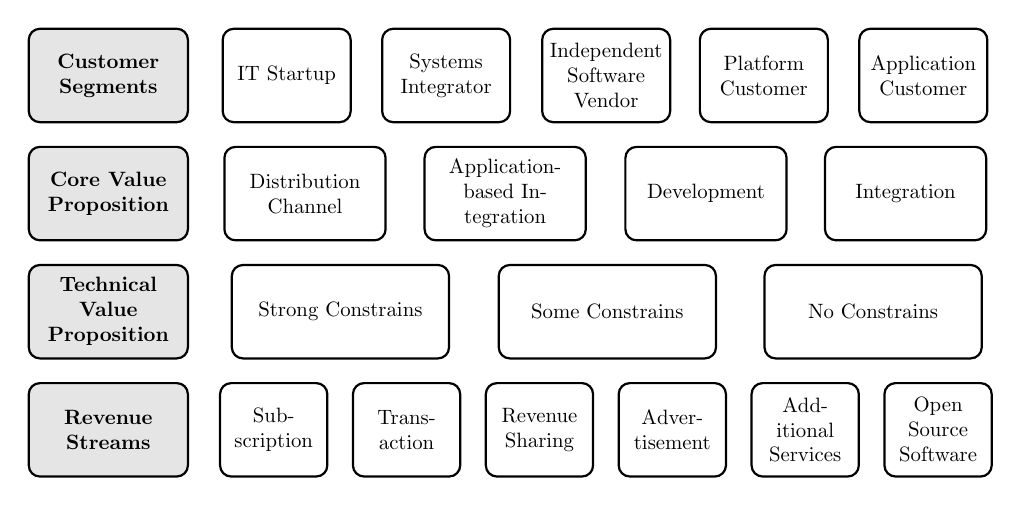
\begin{tikzpicture}[scale=0.75, every node/.style={scale=0.75}]

\node[font={\bfseries},draw,text width=7em,text centered,rectangle,rounded corners,minimum height=4.5em,thick,fill=gray!20] (1) at (0,6) {Customer Segments};
\node[font={\bfseries},draw,text width=7em,text centered,rectangle,rounded corners,minimum height=4.5em,thick,fill=gray!20] (1) at (0,4) {Core Value Proposition};
\node[font={\bfseries},draw,text width=7em,text centered,rectangle,rounded corners,minimum height=4.5em,thick,fill=gray!20] (1) at (0,2) {Technical Value Proposition};
\node[font={\bfseries},draw,text width=7em,text centered,rectangle,rounded corners,minimum height=4.5em,thick,fill=gray!20] (1) at (0,0) {Revenue Streams};

\node[draw,text width=5.5em,text centered,rectangle,rounded corners,minimum height=4.5em,thick] (1) at (3.02,6) {IT Startup};
\node[draw,text width=5.5em,text centered,rectangle,rounded corners,minimum height=4.5em,thick] (1) at (5.72,6) {Systems Integrator};
\node[draw,text width=5.5em,text centered,rectangle,rounded corners,minimum height=4.5em,thick] (1) at (8.43,6) {Independent Software Vendor};
\node[draw,text width=5.5em,text centered,rectangle,rounded corners,minimum height=4.5em,thick] (1) at (11.1,6) {Platform Customer};
\node[draw,text width=5.5em,text centered,rectangle,rounded corners,minimum height=4.5em,thick] (1) at (13.8,6) {Application Customer};

\node[draw,text width=7.1em,text centered,rectangle,rounded corners,minimum height=4.5em,thick] (1) at (3.33,4) {Distribution Channel};
\node[draw,text width=7.1em,text centered,rectangle,rounded corners,minimum height=4.5em,thick] (1) at (6.72,4) {Application-based Integration};
\node[draw,text width=7.1em,text centered,rectangle,rounded corners,minimum height=4.5em,thick] (1) at (10.12,4) {Development};
\node[draw,text width=7.1em,text centered,rectangle,rounded corners,minimum height=4.5em,thick] (1) at (13.5,4) {Integration};

\node[draw,text width=9.8em,text centered,rectangle,rounded corners,minimum height=4.5em,thick] (1) at (3.93,2) {Strong Constrains};
\node[draw,text width=9.8em,text centered,rectangle,rounded corners,minimum height=4.5em,thick] (1) at (8.45,2) {Some Constrains};
\node[draw,text width=9.8em,text centered,rectangle,rounded corners,minimum height=4.5em,thick] (1) at (12.95,2) {No Constrains};

\node[draw,text width=4.5em,text centered,rectangle,rounded corners,minimum height=4.5em,thick] (1) at (2.8,0) {Sub-scription};
\node[draw,text width=4.5em,text centered,rectangle,rounded corners,minimum height=4.5em,thick] (1) at (5.05,0) {Trans-action};
\node[draw,text width=4.5em,text centered,rectangle,rounded corners,minimum height=4.5em,thick] (1) at (7.3,0) {Revenue Sharing};
\node[draw,text width=4.5em,text centered,rectangle,rounded corners,minimum height=4.5em,thick] (1) at (9.55,0) {Adver-tisement};
\node[draw,text width=4.5em,text centered,rectangle,rounded corners,minimum height=4.5em,thick] (1) at (11.8,0) {Add-itional Services};
\node[draw,text width=4.5em,text centered,rectangle,rounded corners,minimum height=4.5em,thick] (1) at (14.05,0) {Open Source Software};

%\node [node, right of=1] (2) {map};

%\node[draw,text width=7em,text centered,rectangle,rounded corners,minimum height=4em,thick] (10) {Customer Segments};
%\node[draw,text width=7em,text centered,rectangle,rounded corners,minimum height=4em,thick,below of=10] (20) {Core Value Proposition};
%\node[draw,text width=7em,text centered,rectangle,rounded corners,minimum height=4em,thick,below of=20] (30) {Technical Value Proposition};
%\node[draw,text width=7em,text centered,rectangle,rounded corners,minimum height=4em,thick,below of=30] (40) {Revenue Streams};

%\node[draw,text width=7em,text centered,rectangle,rounded corners,minimum height=4em,thick,right of=40] (41) {Subscription};
%\node[draw,text width=7em,text centered,rectangle,rounded corners,minimum height=4em,thick,right of=41] (42)  {Transaction};
%\node[draw,text width=7em,text centered,rectangle,rounded corners,minimum height=4em,thick,right of=42] (43) {Revenue Sharing};
%\node[draw,text width=7em,text centered,rectangle,rounded corners,minimum height=4em,thick,right of=43] (44)  {Advertisement};
%\node[draw,text width=7em,text centered,rectangle,rounded corners,minimum height=4em,thick,right of=44] (45)  {Additional Services};
%\node[draw,text width=7em,text centered,rectangle,rounded corners,minimum height=4em,thick,right of=45] (46)  {Open Source Software};

\end{tikzpicture}
	\caption{Classification Scheme for PaaS Business Models}
	\label{fig:cs}
\end{figure}

Based on a comparison of the \ac{PaaS} offerings -- part of the \ac{CVP} within \citet{Johnson2008} business model conceptualization -- four essential and most important core value propositions have been revealed.  First, the core value proposition distribution channel describes the case that a company is opening its ecosystem including the customer base to external stakeholders. These stakeholders -- for instance \acp{ISV} -- in turn will provide additional features to the ecosystem's existing customer base. The Facebook Developers platform is a successful example of a \ac{PaaS} offer focusing on the core value proposition distribution channel. Second, as mentioned above, the \ac{SaaS} layer is already quite mature and well-established within the cloud computing area with a broad range of offered solutions (cf. Appendix \ref{ch:app03}). In order to achieve the demanded customizability of those solution portfolios, it is a common approach that former purely \ac{SaaS} providers extend their offer with \ac{PaaS} capabilities. For instance, the Force.com platform provides the necessary features to customize the Salesforce.com solution portfolio. This group of \ac{PaaS} business models is labeled with the core value proposition application-based integration. Third, another group of \ac{PaaS} platforms are truly dedicated to support the entire application respectively service development process -- including developing, testing, debugging, deploying, and versioning. This core value proposition is simple denoted as development. Well-known examples for development \ac{PaaS} providers respectively platforms are the Google App Engine and Microsoft Windows Azure. And fourth, platforms aiming to integrate any combination of on-premise and on-demand applications as well as systems are characterized by the core value proposition integration. A common case, in which these platforms are used, is the support of complex supply chains between suppliers, producers, and (commercial) consumers. Some of the largest \ac{PaaS} providers respectively platforms are established within this area, like GXS Trading Grid, Compuware Covisint Cloud Engagement Platform, and Dell Boomi.

In alignment with \citet{Tiwana2010}, the governance model of the investigated platforms differs noticeable. Whereas \citet[pp. 679-681]{Tiwana2010} identified the three areas decision right partitioning, control mechanisms, and proprietary vs. shared ownership within platform governance, in the proposed classification scheme a qualitative scale of values is provided -- strictly limited, partly limited, and open. By focusing more on qualitative values, it is possible to support the two classification guidelines user-friendliness as well as economic efficiency. For instance, the Facebook Developers platform maintains a strictly limited governance model, due to fact that the possible options are heavily restricted. On the other side of the scale, platforms like GigaSpaces Cloudify or VMware Cloud Foundry, both are available as open source products, are inherently pursue an open governance model. However, most of the platforms practice a governance model somewhere between these two mentioned extremes (partly limited) and managing the platform in certain parts whereas others are preponderantly shaped by the different customer segments.

Furthermore, the investigated \ac{PaaS} platforms vary remarkable in their technological capabilities. This variety includes among other things programming languages, development environments, frameworks, databases, \acp{API}, and protocols. A quantitative scale of values would not fulfill the classification guidelines, especially the usability of the classification scheme. Therefore, another qualitative scale of values was chosen to represent the technical scope of \ac{PaaS} platforms. Especially \ac{PaaS} platforms focusing on the core value proposition development offer an extensive scope of technological capabilities (for instance Google App Engine and Microsoft Windows Azure) -- denoted within the classification as extensive technical capabilities. Howsoever, all \ac{PaaS} platforms provide at least some rudimentary development possibilities (for instance VMware WaveMaker and LongJump) and labeled as platforms with limited technical capabilities.

The last classification criteria revenue stream \textit{"defines how the company creates value for itself while providing value to the customer"} \citep[p. 53]{Johnson2008}. For the two customer segments platform and application customers subscription and transaction pricing models are prevalent. In case of subscription, the customer pays a regular subscription fee -- commonly a monthly charge -- and gains in reverse the right to use the product for the paid period. The Oracle Java Cloud Service platform is mainly charged through this kind of pricing. Transaction-based price models are usage-dependent, for instance time or processing units, nonetheless paid on a regular base. As common for many \ac{AWS} solutions, also \ac{AWS} Elastic Beanstalk and \ac{AWS} OpsWorks are priced based on certain metrics (in order words transactions). Those both revenue streams are direct revenues and therefore highly pursued by \ac{PaaS} providers. Third-party applications and services are charged by the platform provider or the service provider, however, in both cases the revenue is shared between the two parties. For instance the platforms CloudBees, Salesforce.com Force.com, and SAP HANA Cloud are using this approach to participate in their complementors' success. A common revenue share rate is somewhere between 15\% and 30\% while the platform provider receives obvious the lower amount. A considerable amount of \ac{PaaS} providers offer numerous additional services. These services include among other things trainings, certifications for people, organizations, as well as products respectively applications, advertisements, advisors services, and onboarding packages. Within this research particularly the outstanding offer of services around the platform Salesfore.com Force.com was noticed. All the above mentioned services are subsumed under the heading additional services. Due to the fact that it is not possible to compare the revenue streams onboarding packages and subscription for the simple reason that they represent different levels of significance. However, the revenue streams additional services and subscription can be considered as comparable subject matters. Another revenue stream which seems to be present within the \ac{PaaS} ecosystem is \ac{OSS}. Even though this revenue stream is mainly non-monetary, there are some open source platforms available, for instance GigaSpaces Cloudify and VMware Cloud Foundry. In most cases, the promoting company behind such open source platforms is also offering additional charged services dedicated for those platforms.

Certainly, many more criteria as well as characteristics can be easily added to the classification scheme. Nevertheless, the basic idea was to develop a classification scheme in which hardly any criteria and characteristics can be omitted rather than to develop a comprehensive classification scheme in which no further criteria and characteristics can be added. This idea respectively approach is in alignment with the above briefly mentioned classification guidelines.

\section{Current State of Platform as a Service Providers}\label{ch:sota:cPaaS}

The previously developed classification scheme was used to assess the business models of the 23 investigated \ac{PaaS} providers. Table \ref{tab:cpaas} illustrates how these platforms address the five classification criteria customer segment, core value proposition, governance model, technical scope, and revenue stream. 

During the data gathering process in the beginning of the case study approach as well as in the course of the elaboration of the classification scheme a remarkable number of different terminologies between the investigated \ac{PaaS} providers have been noticed. Almost all providers using their own terms in order to describe their offer, pricing, technological features, as well as stakeholders resp. partners. Especially for the last mentioned term stakeholder an uncountable number of terms exists within the \ac{PaaS} industry. In the following the terms for stakeholders of five exemplary providers are mentioned: technology and service partners \citep{CloudBees2013}; \acp{SI}, \acp{ISV}, and \ac{PaaS} providers \citep{Dell2013}; enterprise partners \citep{OrangeScape2013}; AppExchange and consulting partners \citep{Salesforce.com2013}; as well as strategic, consulting, application, and technology partners \citep{Workday2013}. All these various characteristics have been taken into account and were generalized by means of the above introduced classification scheme within the criterion customer segment. A more standardized terminology could help to improve the user friendliness resp. intelligibility within the \ac{PaaS} industry, but most likely this is difficult to obtain and the marketing shaped terms will remain.

Furthermore the scope as well as shape of the current \ac{PaaS} offers differs noticeable. For example platforms addressing mainly a single customer segment (like \ac{AWS} Elastic Beanstalk, \ac{AWS} OpsWorks, Oracle Java Cloud Service, or VMware Cloud Foundry) are confronted with platforms addressing all five identified customer segments (like LongJump, Salesforce.com Force.com, or SAP HANA Cloud). Also the technical capabilities of the investigated \ac{PaaS} platforms vary remarkable from simple web development platforms (VMware WaveMaker) to powerful development platforms (Microsoft Windows Azure). The application domain which is support by the \ac{PaaS} platform is another distinctive factor -- from platforms supporting a specific application domain (like Dell Boomi and GXS Trading Grid) to platforms rather supporting a broad application domain (like Google App Engine and Microsoft Windows Azure). These findings are in alignment with \citep[p. 5]{Smith2012} and support the statement that the \ac{PaaS} domain is still immature as well as in a developing stage and is located at the so-called \textit{"Peak of Inflated Expectations"}.

Even though it is not possible to generalize any patterns which are prevalent within the set of the 23 analyzed \ac{PaaS} providers -- for the simple reason that this set is by far undersized and therefore not representative -- a few findings are presented below. A majority of the investigated platforms is focusing on the core value proposition development (14 out of 23 investigated \ac{PaaS} platforms). Frequently this core value proposition is accompanied by comprehensive technical features offered by the \ac{PaaS} provider (within this case study research 50\% of the development focused platforms provide powerful technical capabilities), denoted within the classification scheme as extensive technical capabilities. In case the platform is addressing the customer segment \ac{ISV} (18 out of 23 investigated \ac{PaaS} platforms), these customers are often priced in an indirect manner through a revenue share pricing model (28\% of the investigated platforms addressing \acp{ISV} using this pricing model ). End customers -- platform and application customers -- are commonly charged with subscription (52\%), transaction (39\%), or a combination of the prior mentioned pricing models (30\%). Moreover, several \ac{PaaS} providers extend their offering with complementary services (39\%), for instance trainings and certifications, which are summarized as additional services within the classification scheme. Unsurprisingly, all investigated \ac{PaaS} platforms in this case study research addressing the customer segment platform customer and a majority of the platforms addressing the customer segment application customer (57\%).

% ****************************************************************************************************
%Classification of Platform as a Service Providers NEW
% ****************************************************************************************************

\newcolumntype{I}{!{\vrule width 1.3pt}}
\newlength\savedwidth
\newcommand\whline{\noalign{\global\savedwidth\arrayrulewidth
														\global\arrayrulewidth 1.3pt}%
										\hline
										\noalign{\global\arrayrulewidth\savedwidth}}


\begin{longtable}{IL{6.5em}IC{.1cm}|C{.1cm}|C{.1cm}|C{.1cm}|C{.1cm}IC{.1cm}|C{.1cm}|C{.1cm}|C{.1cm}IC{.1cm}|C{.1cm}|C{.1cm}IC{.1cm}|C{.1cm}IC{.1cm}|C{.1cm}|C{.1cm}|C{.1cm}|C{.1cm}I}

\caption{Classification of PaaS Business Models}
\label{tab:cpaas}\\
	
	\whline
		\multirow{2}{6.5em}{\diagbox[height=138pt,width=7.5em]{\scriptsize PaaS\\ \scriptsize Providers}{\scriptsize Classification\\ \scriptsize Scheme}}
		&\multicolumn{5}{C{2.25cm}I}{\scriptsize Customer Segment}
		&\multicolumn{4}{C{1.6cm}I}{\scriptsize Core Value Proposition}
		&\multicolumn{3}{C{1.2cm}I}{\scriptsize Gover-nance Model} 
		&\multicolumn{2}{C{0.7cm}I}{\scriptsize Tech-nical Scope} 
		&\multicolumn{5}{C{2.25cm}I}{\scriptsize Revenue Stream} \\
		\cline{2-20}

		&\begin{sideways}\scriptsize IT Startup\end{sideways} 
		&\begin{sideways}\scriptsize Systems Integrator\end{sideways} 
		&\begin{sideways}\scriptsize Independent Software Vendor\end{sideways} 
		&\begin{sideways}\scriptsize Platform Customer\end{sideways} 
		&\begin{sideways}\scriptsize Application Customer\end{sideways} 
		&\begin{sideways}\scriptsize Distribution Channel\end{sideways} 
		&\begin{sideways}\scriptsize Application-based Integration\end{sideways} 
		&\begin{sideways}\scriptsize Development\end{sideways} 
		&\begin{sideways}\scriptsize Integration\end{sideways} 
		&\begin{sideways}\scriptsize Strictly Limited\end{sideways} 
		&\begin{sideways}\scriptsize Partly Limited\end{sideways} 
		&\begin{sideways}\scriptsize Open\end{sideways} 
		&\begin{sideways}\scriptsize Limited Technical Capabilities\end{sideways} 
		&\begin{sideways}\scriptsize Extensive Technical Capabilities~~~\end{sideways} 
		&\begin{sideways}\scriptsize Subscription\end{sideways} 
		&\begin{sideways}\scriptsize Transaction\end{sideways} 
		&\begin{sideways}\scriptsize Revenue Sharing\end{sideways} 
		&\begin{sideways}\scriptsize Additional Services\end{sideways} 
		&\begin{sideways}\scriptsize Open Source Software\end{sideways} \\
		\hline
	
	\endfirsthead
	\whline  
	\multicolumn{20}{IlI}{\scriptsize \textit{continued from previous page (Classification of PaaS Business Models)}}\\ 
	\whline
	\multirow{2}{6.5em}{\diagbox[height=138pt,width=7.5em]{\scriptsize PaaS\\ \scriptsize Providers}{\scriptsize Classification\\ \scriptsize Scheme}}
		&\multicolumn{5}{C{2.25cm}I}{\scriptsize Customer Segment}
		&\multicolumn{4}{C{1.6cm}I}{\scriptsize Core Value Proposition}
		&\multicolumn{3}{C{1.2cm}I}{\scriptsize Gover-nance Model} 
		&\multicolumn{2}{C{0.7cm}I}{\scriptsize Tech-nical Scope} 
		&\multicolumn{5}{C{2.25cm}I}{\scriptsize Revenue Stream} \\
		\cline{2-20}

		&\begin{sideways}\scriptsize IT Startup\end{sideways} 
		&\begin{sideways}\scriptsize Systems Integrator\end{sideways} 
		&\begin{sideways}\scriptsize Independent Software Vendor\end{sideways} 
		&\begin{sideways}\scriptsize Platform Customer\end{sideways} 
		&\begin{sideways}\scriptsize Application Customer\end{sideways} 
		&\begin{sideways}\scriptsize Distribution Channel\end{sideways} 
		&\begin{sideways}\scriptsize Application-based Integration\end{sideways} 
		&\begin{sideways}\scriptsize Development\end{sideways} 
		&\begin{sideways}\scriptsize Integration\end{sideways} 
		&\begin{sideways}\scriptsize Strictly Limited\end{sideways} 
		&\begin{sideways}\scriptsize Partly Limited\end{sideways} 
		&\begin{sideways}\scriptsize Open\end{sideways} 
		&\begin{sideways}\scriptsize Limited Technical Capabilities\end{sideways} 
		&\begin{sideways}\scriptsize Extensive Technical Capabilities~~~\end{sideways} 
		&\begin{sideways}\scriptsize Subscription\end{sideways} 
		&\begin{sideways}\scriptsize Transaction\end{sideways} 
		&\begin{sideways}\scriptsize Revenue Sharing\end{sideways} 
		&\begin{sideways}\scriptsize Additional Services\end{sideways} 
		&\begin{sideways}\scriptsize Open Source Software\end{sideways} \\
	\hline
	\endhead
	\hline
	\multicolumn{20}{IrI}{\scriptsize \textit{continued on next page}}\\
	\whline
	\endfoot
	\whline
	\endlastfoot

\scriptsize AWS Elastic Beanstalk &
	% Customer Segments
	& & & \scriptsize x& & 
	% Core Value Proposition
	& & \scriptsize x& &
	% Governance Model
	& & \scriptsize x& 
	% Technical Scope
	& \scriptsize x&
	% Revenue Stream
	& \scriptsize x& & &  \\\hline

\scriptsize AWS OpsWorks &
	% Customer Segments
	& & & \scriptsize x& & 
	% Core Value Proposition
	& & \scriptsize x& &
	% Governance Model
	& & \scriptsize x& 
	% Technical Scope
	& \scriptsize x& 
	% Revenue Stream
	& \scriptsize x& & &  \\\hline

\scriptsize \scriptsize Caspio Bridge &
	% Customer Segments
	\scriptsize x& & \scriptsize x& \scriptsize x& \scriptsize x&
	% Core Value Proposition
	& & \scriptsize x& & 
	% Governance Model
	& \scriptsize x& & 
	% Technical Scope
	\scriptsize x& & 
	% Revenue Stream
	\scriptsize x& \scriptsize x& & \scriptsize x&  \\\hline

\scriptsize CloudBees &
	% Customer Segments
	\scriptsize x& \scriptsize x& \scriptsize x& \scriptsize x& & 
	% Core Value Proposition
	& & \scriptsize x& &
	% Governance Model
	& & \scriptsize x& 
	% Technical Scope
	& \scriptsize x&
	% Revenue Stream
	\scriptsize x& \scriptsize x& \scriptsize x& \scriptsize x&  \\\hline

\scriptsize Compuware Covisint Cloud Engagement &
	% Customer Segments
	& & \scriptsize x& \scriptsize x& \scriptsize x& 
	% Core Value Proposition
	& & & \scriptsize x&
	% Governance Model
	& \scriptsize x& & 
	% Technical Scope
	\scriptsize x& &
	% Revenue Stream
	\multicolumn{5}{C{0.75cm}I}{\scriptsize n/a}  \\\hline

\scriptsize Dell Boomi &
	% Customer Segments
	& \scriptsize x& \scriptsize x& \scriptsize x& &
	% Core Value Proposition
	& & & \scriptsize x& 
	% Governance Model
	& \scriptsize x& & 
	% Technical Scope
	& \scriptsize x&
	% Revenue Stream
	\scriptsize x& & & \scriptsize x&  \\\hline

\scriptsize Facebook Developers &
	% Customer Segments
	\scriptsize x& & \scriptsize x& \scriptsize x& \scriptsize x& 
	% Core Value Proposition
	\scriptsize x& & & &
	% Governance Model
	\scriptsize x& & & 
	% Technical Scope
	& \scriptsize x&
	% Revenue Stream
	& & \scriptsize x& \scriptsize x&  \\\hline

\scriptsize GigaSpaces Cloudify &
	% Customer Segments
	\scriptsize x& & \scriptsize x& \scriptsize x& & 
	% Core Value Proposition
	& & \scriptsize x& &
	% Governance Model
	& & \scriptsize x& 
	% Technical Scope
	\scriptsize x& &
	% Revenue Stream
	& & & \scriptsize x& \scriptsize x  \\\hline

\scriptsize Google App Engine &
	% Customer Segments
	\scriptsize x& & \scriptsize x& \scriptsize x& \scriptsize x& 
	% Core Value Proposition
	& & \scriptsize x & &
	% Governance Model
	& \scriptsize x& & 
	% Technical Scope
	& \scriptsize x&
	% Revenue Stream
	\scriptsize x& \scriptsize x& & &  \\\hline

\scriptsize GXS Trading Grid &
	% Customer Segments
	& \scriptsize x& \scriptsize x& \scriptsize x& & 
	% Core Value Proposition
	& & & \scriptsize x&
	% Governance Model
	& \scriptsize x& & 
	% Technical Scope
	& \scriptsize x&
	% Revenue Stream
	\scriptsize x& & & &  \\\hline

\scriptsize IBM SmartCloud Application Services &
	% Customer Segments
	& \scriptsize x& \scriptsize x& \scriptsize x& \scriptsize x& 
	% Core Value Proposition
	& & \scriptsize x& &
	% Governance Model
	& \scriptsize x& & 
	% Technical Scope
	& \scriptsize x& 
	% Revenue Stream
	\scriptsize x& \scriptsize x& & \scriptsize x&  \\\hline
	
\scriptsize LongJump &
	% Customer Segments
	\scriptsize x& \scriptsize x& \scriptsize x& \scriptsize x& \scriptsize x& 
	% Core Value Proposition
	& & \scriptsize x& &
	% Governance Model
	& \scriptsize x& & 
	% Technical Scope
	\scriptsize x& &
	% Revenue Stream
	\scriptsize x& \scriptsize x& & &  \\\hline

\scriptsize Microsoft Windows Azure &
	% Customer Segments
	& \scriptsize x& \scriptsize x& \scriptsize x& \scriptsize x&
	% Core Value Proposition
	& & \scriptsize x& & 
	% Governance Model
	& \scriptsize x& & 
	% Technical Scope
	& \scriptsize x& 
	% Revenue Stream
	\scriptsize x& \scriptsize x& \scriptsize x& &  \\\hline

\scriptsize NetSuite SuiteCloud &
	% Customer Segments
	& \scriptsize x& \scriptsize x& \scriptsize x& \scriptsize x& 
	% Core Value Proposition
	& \scriptsize x& & &
	% Governance Model
	& \scriptsize x& & 
	% Technical Scope
	& \scriptsize x&
	% Revenue Stream
	\multicolumn{5}{C{0.75cm}I}{\scriptsize n/a}  \\\hline

\scriptsize Oracle Java Cloud Service &
	% Customer Segments
	& & & \scriptsize x& & 
	% Core Value Proposition
	& & \scriptsize x& &
	% Governance Model
	& \scriptsize x& & 
	% Technical Scope
	\scriptsize x& &
	% Revenue Stream
	\scriptsize x& & & &  \\\hline

\scriptsize OrangeScape Cloud &
	% Customer Segments
	& & & \scriptsize x& & 
	% Core Value Proposition
	& & \scriptsize x& &
	% Governance Model
	& \scriptsize x& & 
	% Technical Scope
	\scriptsize x& &
	% Revenue Stream
	\multicolumn{5}{C{0.75cm}I}{\scriptsize n/a}  \\\hline

\scriptsize RightScale MultiCloud Platform &
	% Customer Segments
	\scriptsize x& & \scriptsize x& \scriptsize x& \scriptsize x& 
	% Core Value Proposition
	& & \scriptsize x& &
	% Governance Model
	& \scriptsize x& & 
	% Technical Scope
	\scriptsize x& &
	% Revenue Stream
	\scriptsize x& \scriptsize x& &\scriptsize x &  \\\hline

\scriptsize Salesforce.com Force.com &
	% Customer Segments
	\scriptsize x& \scriptsize x& \scriptsize x& \scriptsize x& \scriptsize x& 
	% Core Value Proposition
	& \scriptsize x& & &
	% Governance Model
	& \scriptsize x& & 
	% Technical Scope
	& \scriptsize x& 
	% Revenue Stream
	\scriptsize x& & \scriptsize x& \scriptsize x&  \\\hline

\scriptsize SAP HANA Cloud &
	% Customer Segments
	\scriptsize x& \scriptsize x& \scriptsize x& \scriptsize x& \scriptsize x&
	% Core Value Proposition
	& & & \scriptsize x& 
	% Governance Model
	& \scriptsize x& & 
	% Technical Scope
	\scriptsize x& & 
	% Revenue Stream
	\scriptsize x& & \scriptsize x& \scriptsize x&  \\\hline

\scriptsize TIBCO Silver &
	% Customer Segments
	& \scriptsize x& \scriptsize x& \scriptsize x& \scriptsize x&
	% Core Value Proposition
	& \scriptsize x& & & 
	% Governance Model
	& \scriptsize x& & 
	% Technical Scope
	& \scriptsize x&
	% Revenue Stream
	\multicolumn{5}{C{0.75cm}I}{\scriptsize n/a}  \\\hline

\scriptsize VMware Cloud Foundry &
	% Customer Segments
	& & & \scriptsize x& & 
	% Core Value Proposition
	& & \scriptsize x& &
	% Governance Model
	& & \scriptsize x& 
	% Technical Scope
	& \scriptsize x&
	% Revenue Stream
	\multicolumn{4}{C{0.6cm}|}{\scriptsize n/a} & \scriptsize x \\\hline

\scriptsize VMware WaveMaker &
	% Customer Segments
	\scriptsize x& & \scriptsize x& \scriptsize x& & 
	% Core Value Proposition
	& & \scriptsize x& &
	% Governance Model
	& & \scriptsize x& 
	% Technical Scope
	\scriptsize x& &
	% Revenue Stream
	& & & &\scriptsize x  \\\hline

\scriptsize Workday Integration Cloud &
	% Customer Segments
	& \scriptsize x& \scriptsize x& \scriptsize x& \scriptsize x&
	% Core Value Proposition
	& \scriptsize x& & & 
	% Governance Model
	& \scriptsize x& & 
	% Technical Scope
	\scriptsize x& &
	% Revenue Stream
	\multicolumn{5}{C{0.75cm}I}{\scriptsize n/a}  \\\hline

\end{longtable}